\lhead{Capítulo \ref{ch_4}}
\rhead{\newtitle}
\cfoot{\thepage}
\renewcommand{\headrulewidth}{1pt}
\renewcommand{\footrulewidth}{1pt}

\chapter{Diseño del Sistema de Información}\label{ch_4}
\noindent El objetivo del proceso de Diseño del Sistema de Información (DSI) es la definición de la arquitectura del sistema y del entorno tecnológico que le va a dar soporte, junto con la especificación detallada de los componentes del sistema de información.\\

\noindent A partir de dicha información, se generan todas las especificaciones de construcción relativas al propio sistema, así como la descripción técnica del plan de pruebas, la definición de los requisitos de implantación y el diseño de los procedimientos de migración y carga inicial,éstos últimos cuando proceda.\\

\noindent En la actividad Definición de la Arquitectura del Sistema, se establece el particionamiento físico del sistema de información, así como su organización en subsistemas de diseño, la especificación del entorno tecnológico, y sus requisitos de operación, administración, seguridad y control de acceso. Se completan los catálogos de requisitos y normas, en función de la definición del entorno tecnológico, con aquellos aspectos relativos al diseño y construcción que sea necesario contemplar. Asimismo, se crea un catálogo de excepciones del sistema, en el que se registran las situaciones de funcionamiento secundario o anómalo que se estime oportuno considerar y, por lo tanto, diseñar y probar. Este catálogo de excepciones se utiliza como referencia en la especificación técnica de las pruebas del sistema.
\section{Definición de niveles de arquitectura.}

\begin{figure}[H]
    \centering
    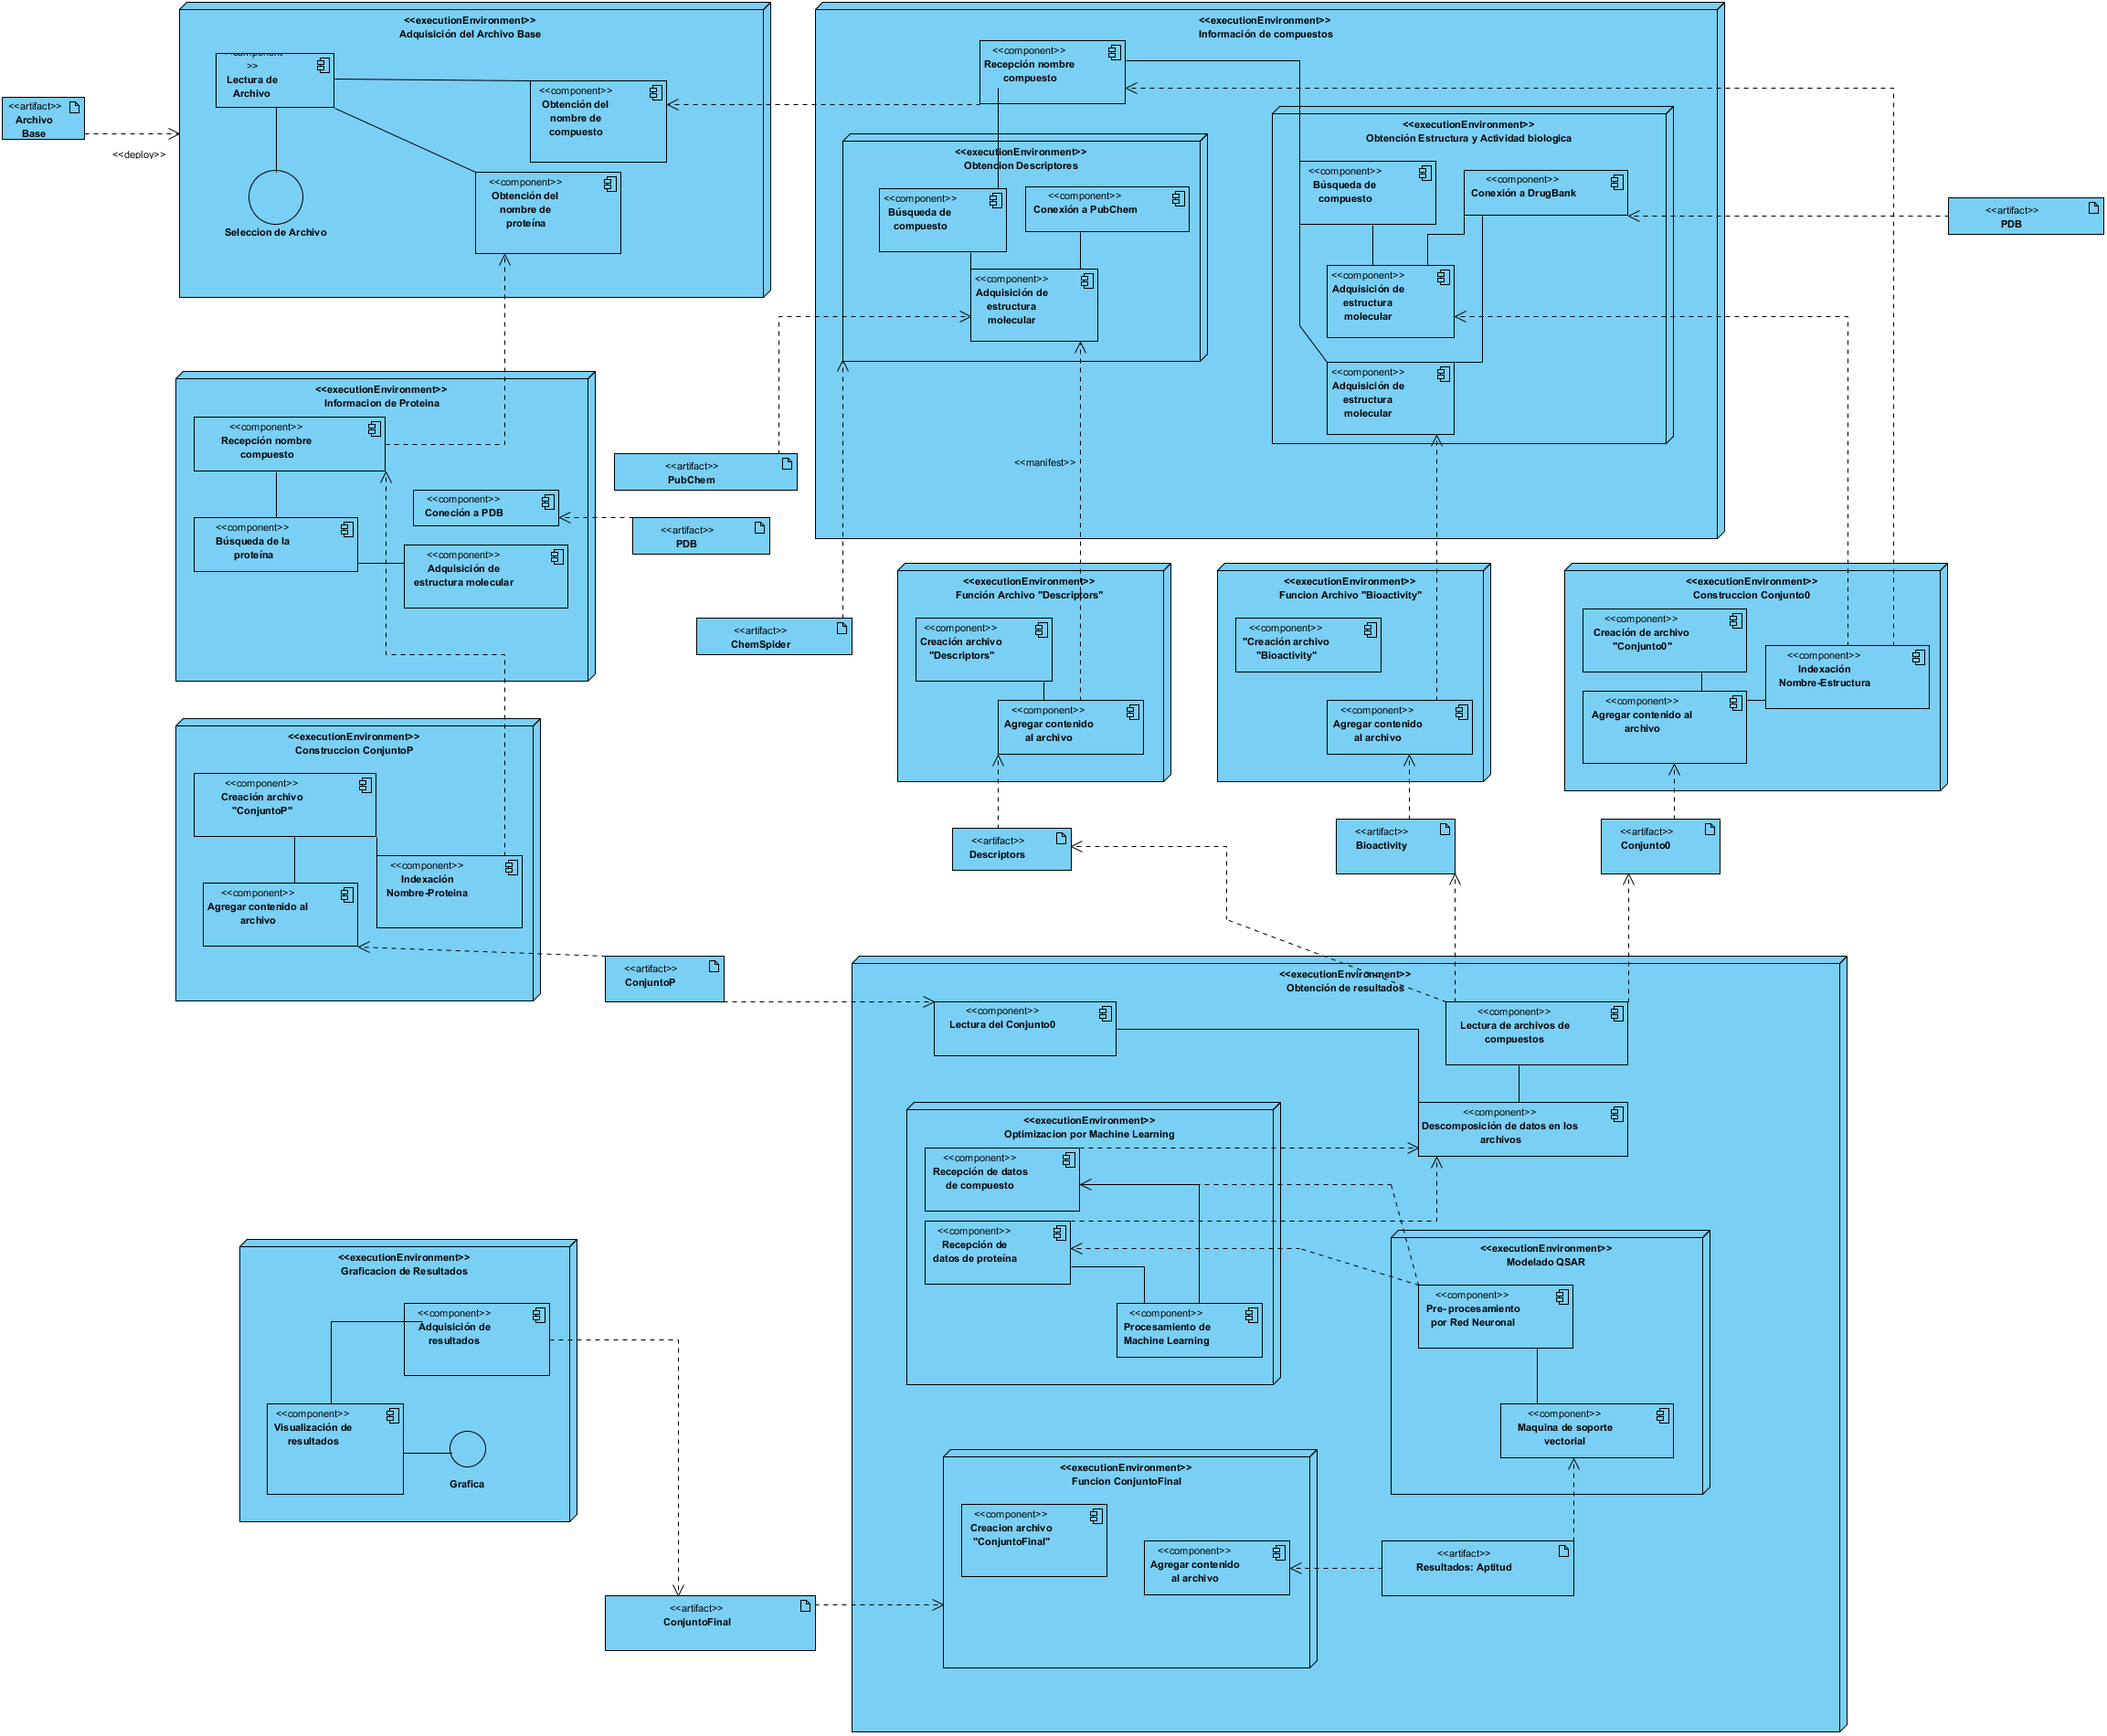
\includegraphics[scale=0.25]{Capitulo3/images/Niveles_de_Arquitectura.png}
    \caption{Niveles de Arquitectura}
    \label{arquitectura_N}
\end{figure}
\newpage

\section{Identificación de Requisitos de Diseño}
\noindent Se realiza la especificación de los requisitos que están directamente relacionados con la adopción o diseño de la arquitectura, y que pueden condicionar el diseño o la construcción del sistema de información.
% Please add the following required packages to your document preamble:
% \usepackage{multirow}
% \usepackage{longtable}
% Note: It may be necessary to compile the document several times to get a multi-page table to line up properly
\begin{longtable}{|l|l|l|l|}
\caption{Identificación de Requisitos de Diseño}
\label{req_dis}\\
\hline
\textbf{\begin{tabular}[c]{@{}l@{}}Módulo de \\ Arquitectura\end{tabular}}              & \textbf{\begin{tabular}[c]{@{}l@{}}Sub-Módulo de \\ Arquitectura\end{tabular}}                                                                                                                                                                                                  & \textbf{\begin{tabular}[c]{@{}l@{}}Requerimiento \\ Funcional\end{tabular}}                                                                 & \textbf{Descripción}                                                                                                                                                                                                                                                                                                                                           \\ \hline
\endfirsthead
%
\multicolumn{4}{c}%
{{\bfseries Tabla \thetable\ Continuación de la página anterior.}} \\
\endhead
%
\begin{tabular}[c]{@{}l@{}}Adquisición\\ de Archivo\\ Base\end{tabular}                 & \begin{tabular}[c]{@{}l@{}}- Lectura de\\ archivo\\ \\ - Selección de\\ archivo.\end{tabular}                                                                                                                                                                                   & \begin{tabular}[c]{@{}l@{}}Requerimiento\\ Funcional 1.1:\\ Obtención y\\ lectura del\\ archivo base.\end{tabular}                          & \begin{tabular}[c]{@{}l@{}}El sistema recibe del\\ usuario un archivo de\\ texto plano en el cual se\\ tiene una lista con los\\ nombres de los\\ compuestos y nombres\\ de las proteínas de la\\ patología que forman\\ parte del objeto de\\ estudio.\end{tabular}                                                                                           \\ 
\multirow{}{}{\begin{tabular}[c]{@{}l@{}}Información\\ de\\ compuestos.\end{tabular}} & \begin{tabular}[c]{@{}l@{}}- Recepción\\ nombre de\\ compuesto.\\ \\ - Obtención de\\ estructura y\\ actividad\\ biológica.\\ \\ - Conexión a\\ DrugBank.\\ \\ -Búsqueda del\\ compuesto.\\ \\ - Adquisición de\\ Estructura\\ molecular.\end{tabular}                          & \begin{tabular}[c]{@{}l@{}}Requerimiento\\ Funcional 1.2:\\ Búsqueda de\\ los compuestos\\ indicados.\end{tabular}                          & \begin{tabular}[c]{@{}l@{}}Por cada elemento de la\\ lista de compuestos en\\ el archivo ingresado por\\ el usuario, el sistema los\\ buscará en la base de\\ datos en línea\\ “DrugBank”.\end{tabular}                                                                                                                                                        \\ \cline{2-4} 
                                                                                        & \begin{tabular}[c]{@{}l@{}}- Recepción\\ nombre de\\ compuesto.\\ \\ - Obtención de\\ estructura y\\ actividad\\ biológica.\\ \\ - Conexión a\\ PubChem.\\ \\ - Conexión a\\ ChemSpider.\\ \\ - Búsqueda del\\ compuesto.\\ \\ -Adquisición de\\ los descriptores.\end{tabular} & \begin{tabular}[c]{@{}l@{}}Requerimiento\\ Funcional 1.3:\\ Búsqueda de\\ los descriptores\\ de los\\ compuestos.\end{tabular}              & \begin{tabular}[c]{@{}l@{}}El sistema, utilizando\\ como referencia la lista\\ de compuestos\\ ingresada por el usuario,\\ realiza una búsqueda de\\ los descriptores físico\\ químicos por cada uno\\ de los elementos de\\ dicha lista en la base de\\ datos “PubChem” y\\ ChemSpider.\end{tabular}                                                          \\ \cline{2-4} 
                                                                                        & \begin{tabular}[c]{@{}l@{}}- Recepción\\ nombre de\\ compuesto.\\ \\ - Obtención de\\ estructura y\\ actividad\\ biológica.\\ \\ - Conexión a\\ DrugBank.\\ \\ - Búsqueda del\\ compuesto.\\ \\ - Adquisición de la\\ actividad\\ biológica.\end{tabular}                       & \begin{tabular}[c]{@{}l@{}}Requerimiento\\ Funcional 1.4:\\ Búsqueda de\\ los mecanismos\\ de acción de los\\ compuestos.\end{tabular}      & \begin{tabular}[c]{@{}l@{}}El sistema, utilizando\\ como referencia la lista\\ de compuestos\\ ingresada por el usuario,\\ realiza la búsqueda de\\ los mecanismos de\\ acción por cada uno de\\ los elementos de dicha\\ lista en la base de datos\\ “DrugBank”.\end{tabular}                                                                                 \\ \hline
\begin{tabular}[c]{@{}l@{}}Información\\ de proteína.\end{tabular}                      & \begin{tabular}[c]{@{}l@{}}- Recepción\\ nombre proteína.\\ \\ - Conexión a PDB.\\ \\ - Búsqueda de la\\ proteína.\\ \\ - Adquisición de\\ estructura\\ molecular.\end{tabular}                                                                                                 & \begin{tabular}[c]{@{}l@{}}Requerimiento\\ Funcional 1.5:\\ Búsqueda de\\ las proteínas\\ indicadas.\end{tabular}                           & \begin{tabular}[c]{@{}l@{}}Por cada elemento de la\\ lista de proteínas en el\\ archivo ingresado por el\\ usuario, el sistema las\\ buscará en la base de\\ datos en línea “PDB”.\end{tabular}                                                                                                                                                                \\ \hline
\begin{tabular}[c]{@{}l@{}}Información\\ de Proteína.\end{tabular}                      & \begin{tabular}[c]{@{}l@{}}Adquisición de\\ estructura\\ molecular\\ proteína.\end{tabular}                                                                                                                                                                                     & \multirow{}{}{\begin{tabular}[c]{@{}l@{}}Requerimiento\\ Funcional 1.6:\\ Confirmación de\\ los resultados\\ de la búsqueda\end{tabular}} & \multirow{}{}{\begin{tabular}[c]{@{}l@{}}El sistema presenta al\\ usuario los resultados\\ de la búsqueda y este\\ último valida que sean\\ correctos.\end{tabular}}                                                                                                                                                                                         \\ \cline{1-2}
\begin{tabular}[c]{@{}l@{}}Información\\ de\\ Compuestos.\end{tabular}                  & \begin{tabular}[c]{@{}l@{}}- Adquisición de\\ estructura\\ molecular\\ compuesto\\ \\ \\ - Adquisición de\\ descriptores.\\ \\ \\ - Adquisición de\\ mecanismos de\\ acción.\end{tabular}                                                                                       &                                                                                                                                             &                                                                                                                                                                                                                                                                                                                                                                \\ \hline
\begin{tabular}[c]{@{}l@{}}Función\\ Archivo\\ “Descriptors”\end{tabular}               & \begin{tabular}[c]{@{}l@{}}- Creación archivo\\ descriptors.\\ \\ - Agregar\\ contenido al\\ archivo.\end{tabular}                                                                                                                                                              & \multirow{}{}{\begin{tabular}[c]{@{}l@{}}Requerimiento\\ Funcional 1.7:\\ Construcción de\\ conjuntos.\end{tabular}}                      & \multirow{}{}{\begin{tabular}[c]{@{}l@{}}El sistema organiza la\\ información recabada\\ durante el proceso de\\ búsqueda, en archivos\\ con estructuras\\ definidas, denominados\\ conjuntos, que permiten\\ continuar a la fase de\\ procesamiento de\\ información.\end{tabular}}                                                                         \\ \cline{1-2}
\begin{tabular}[c]{@{}l@{}}Función\\ Archivo\\ “BioActivity”\end{tabular}               & \begin{tabular}[c]{@{}l@{}}- Creación archivo\\ bioactivity.\\ \\ - Agregar\\ contenido al\\ archivo.\end{tabular}                                                                                                                                                              &                                                                                                                                             &                                                                                                                                                                                                                                                                                                                                                                \\ \hline
\begin{tabular}[c]{@{}l@{}}Construcción \\ Conjunto0\end{tabular}                       & \begin{tabular}[c]{@{}l@{}}- Creación archivo\\ Conjunto0.\\ \\ - Indexación\\ Nombre-Estructura.\\ \\ - Agregar\\ contenido al\\ archivo.\end{tabular}                                                                                                                         & \begin{tabular}[c]{@{}l@{}}Requerimiento\\ Funcional 1.7.1:\\ Construcción\\ del conjunto0\end{tabular}                                     & \begin{tabular}[c]{@{}l@{}}El sistema agrupa los\\ datos de los\\ compuestos (nombre,\\ estructura molecular,\\ mecanismos de acción)\\ en un conjunto de\\ archivos denominado\\ conjunto 0.\end{tabular}                                                                                                                                                     \\ \hline
\begin{tabular}[c]{@{}l@{}}Construcción \\ ConjuntoP\end{tabular}                       & \begin{tabular}[c]{@{}l@{}}- Creación archivo\\ Conjunto0.\\ \\ - Indexación\\ Nombre-Estructura.\\ \\ - Agregar\\ contenido al\\ archivo.\end{tabular}                                                                                                                         & \begin{tabular}[c]{@{}l@{}}Requerimiento\\ Funcional 1.7.2:\\ Construcción\\ del conjuntoP\end{tabular}                                     & \begin{tabular}[c]{@{}l@{}}El sistema agrupa la\\ información de la(s)\\ proteína(s) (nombre de\\ la proteína, estructura\\ molecular de la\\ proteína) de la patología\\ indicada por el usuario,\\ en un archivo\\ denominado conjunto P.\end{tabular}                                                                                                       \\ \hline
\multirow{4}{*}{\begin{tabular}[c]{@{}l@{}}Obtención\\ de\\ Resultados.\end{tabular}}   & \begin{tabular}[c]{@{}l@{}}- Lectura del\\ conjunto0\\ \\ - Descomposición\\ de archivo para\\ datos.\\ \\ - Recepción de\\ datos de\\ compuesto.\end{tabular}                                                                                                                  & \begin{tabular}[c]{@{}l@{}}Requerimiento\\ Funcional 2.1:\\ Adquisición y\\ descomposición\\ del conjunto0.\end{tabular}                    & \begin{tabular}[c]{@{}l@{}}El sistema lee el\\ conjunto 0 (previamente\\ definido)\\ correspondiente a un\\ compuesto, para\\ descomponerlo y \\ obtener nombre,\\ descriptores , estructura\\ molecular y mecanismos\\ de acción.\end{tabular}                                                                                                                \\ \cline{2-4} 
                                                                                        & \begin{tabular}[c]{@{}l@{}}- Lectura del\\ conjuntoP\\ \\ - Descomposición\\ de archivo para\\ datos.\\ \\ - Recepción de\\ datos de la\\ proteína.\end{tabular}                                                                                                                & \begin{tabular}[c]{@{}l@{}}Requerimiento \\ Funcional 2.2:\\ Adquisición y\\ descomposición\\ del conjuntoP.\end{tabular}                   & \begin{tabular}[c]{@{}l@{}}El sistema consigue el\\ nombre de la proteína\\ de interés así como su\\ estructura molecular\\ esta información\\ proveniente del conjunto P.\end{tabular}                                                                                                                                                                        \\ \cline{2-4} 
                                                                                        & \begin{tabular}[c]{@{}l@{}}Optimización\\ por Machine\\ Learning\end{tabular}                                                                                                                                                                                                   & \begin{tabular}[c]{@{}l@{}}Requerimiento\\ Funcional 2.3:\\ Método de\\ Machine\\ Learning\\  para\\ optimización.\end{tabular}             & \begin{tabular}[c]{@{}l@{}}El sistema,   a través de\\ este módulo trabaja  con\\ los datos\\ correspondientes al\\ compuesto  y proteína\\ con el objetivo de\\ optimizar la obtención\\ de resultados.\end{tabular}                                                                                                                                          \\ \cline{2-4} 
                                                                                        & \begin{tabular}[c]{@{}l@{}}- Modelado QSAR\\ \\ -Pre-procesamiento \\ por redes \\ neuronales\\ \\  - Maquina de\\ soporte vectorial\end{tabular}                                                                                                                               & \begin{tabular}[c]{@{}l@{}}Requerimiento\\ Funcional 2.4:\\ Modelado\\ QSAR.\end{tabular}                                                   & \begin{tabular}[c]{@{}l@{}}El sistema producirá\\ con los datos\\ pertenecientes a la\\ proteína y  compuesto\\ de interés  el modelo\\ QSAR propio de la\\ actividad farmacológica\\ entre el fármaco y la\\ proteína objetivo.\end{tabular}                                                                                                                  \\ \hline
\begin{tabular}[c]{@{}l@{}}Graficación\\ de\\ resultados.\end{tabular}                  & \begin{tabular}[c]{@{}l@{}}Adquisición de\\ resultados.\end{tabular}                                                                                                                                                                                                            & \begin{tabular}[c]{@{}l@{}}Requerimiento\\ Funcional 3.1:\\ Lectura y\\ ordenamiento\\ del conjunto\\ final.\end{tabular}                   & \begin{tabular}[c]{@{}l@{}}El sistema recibe el\\ conjunto final que\\ contiene el nombre del\\ compuesto y la  aptitud,\\ dicha información será\\ leída y ordena del más\\ apto al menos apto para\\ enfrentar la proteína de\\ la  patología indicada. A\\ la salida se tiene un\\ archivo de texto plano\\ que contiene una lista\\ ordenada.\end{tabular} \\ \hline
                                                                                        & \begin{tabular}[c]{@{}l@{}}Visualización de\\ resultados.\end{tabular}                                                                                                                                                                                                          & \begin{tabular}[c]{@{}l@{}}Requerimiento\\ Funcional 3.2:\\ Diseño gráfico\\ de resultados.\end{tabular}                                    & \begin{tabular}[c]{@{}l@{}}El sistema obtiene el\\ archivo que contiene la\\ lista ordenada  la cual\\ será utilizada para\\ desplegar de manera\\ gráfica  al usuario.\end{tabular}                                                                                                                                                                           \\ \hline
\end{longtable}

\newpage
%%%%%%%%%%%%%%%%%%%%%%%%%%%%%%%%%%%%%%%%%5
\section{Especificación de Excepciones}
\noindent El objetivo de esta tarea es la definición de los comportamientos no habituales en el
sistema, que reflejan situaciones anómalas o secundarias en el funcionamiento y ejecución del
sistema de información. Para ello, se establece previamente el nivel de especificación de las
mismas, así como los criterios de catalogación y clasificación.
Se propone su catalogación como ayuda para el diseño del sistema de información y
como guía en la especificación técnica de las pruebas, al permitir la generación de algunos
casos de prueba de forma inmediata. Dicho catálogo se va completando a partir de las
actividades correspondientes al diseño detallado de los subsistemas.\\

Las excepciones se describen incluyendo, al menos, los siguientes conceptos:\\

\begin{itemize}
    \item Tipo y descripción de la excepción.
    \item Condiciones previas del sistema de información.
    \item Elemento afectado (nodo, módulo, caso de uso).
    \item Respuesta del sistema de información.
    \item Elemento asociado a la respuesta esperada del sistema (módulo, clase, procedimiento,etc.).
\end{itemize}

%%%%%%%%%%%%%%%%%%%%%%%%%%%%%%%%%5
% Please add the following required packages to your document preamble:
% \usepackage{longtable}
% Note: It may be necessary to compile the document several times to get a multi-page table to line up properly
\begin{longtable}{|l|l|l|l|l|}
\caption{Catalogo de Excepciones}
\label{catalogo_de_excepciones}\\
\hline
\textbf{ID} & \textbf{\begin{tabular}[c]{@{}l@{}}Nombre de\\ Excepción\end{tabular}}                        & \textbf{Descripción}                                                                                                                                                                                                                                                           & \textbf{\begin{tabular}[c]{@{}l@{}}Ubicación\\ (Requerimiento)\end{tabular}}                                      & \textbf{\begin{tabular}[c]{@{}l@{}}Elemento\\ afectado\end{tabular}} \\ \hline
\endfirsthead
%
\multicolumn{5}{c}%
{{\bfseries Tabla \thetable\ Continuación de la página anterior}} \\
\endhead
%
EX1         & \begin{tabular}[c]{@{}l@{}}Excepción  \\ lectura del \\ archivo base.\end{tabular}            & \begin{tabular}[c]{@{}l@{}}Excepción que se \\ genera al \\ presentarse \\ un error de en \\ adquisición del \\ archivo base:\\ - No se encuentra \\ el archivo.\\ - El archivo está \\ corrompido o \\ incompleto.\end{tabular}                                               & \begin{tabular}[c]{@{}l@{}}RF1.1: \\ Obtención \\ y lectura del \\ archivo base.\end{tabular}                     & \begin{tabular}[c]{@{}l@{}}Archivo \\ base.\end{tabular}             \\ \hline
EX2         & \begin{tabular}[c]{@{}l@{}}Excepción de \\ formato de \\ datos.\end{tabular}                  & \begin{tabular}[c]{@{}l@{}}Excepción de error \\ de los datos \\ existentes en\\ el archivo base.\\ - No es posible la\\ adquisición del \\ nombre de \\ compuesto o\\ proteína.\\ - El  dato adquirido \\ no tiene sentido \\ con lo que debe de \\ representar.\end{tabular} & \begin{tabular}[c]{@{}l@{}}RF1.1: \\ Obtención y\\ lectura del \\ archivo base.\end{tabular}                      & \begin{tabular}[c]{@{}l@{}}Nombre \\ del\\ compuesto.\end{tabular}   \\ \hline
EX3         & \begin{tabular}[c]{@{}l@{}}Excepción de\\ conexión a\\ DrugBank\end{tabular}                  & \begin{tabular}[c]{@{}l@{}}Excepción que \\ indica error en \\ la conexión a\\ las bases de datos.\\ - Error de conexión\\  a DrugBank\end{tabular}                                                                                                                            & \begin{tabular}[c]{@{}l@{}}RF1.2: \\ Búsqueda de\\ los compuestos\\ indicados.\end{tabular}                       & \begin{tabular}[c]{@{}l@{}}Archivo\\ “Conjunto0”\end{tabular}        \\ \hline
EX4         & \begin{tabular}[c]{@{}l@{}}Excepción\\ Compuesto no\\ encontrado.\end{tabular}                & \begin{tabular}[c]{@{}l@{}}Excepción que \\ notifica que no \\ existe el\\ compuesto en\\ DrugBank.\\ - Error\\ compuesto\\ inexistente.\end{tabular}                                                                                                                          & \begin{tabular}[c]{@{}l@{}}RF1.2: \\ Búsqueda de\\ los compuestos\\ indicados.\end{tabular}                       & \begin{tabular}[c]{@{}l@{}}Archivo\\ “Conjunto0”\end{tabular}        \\ \hline
EX5         & \begin{tabular}[c]{@{}l@{}}Excepción no se \\ puede obtener \\ datos.\end{tabular}            & \begin{tabular}[c]{@{}l@{}}Excepción que \\ indica que no \\ se pudo adquirir\\ información.\\ - Error de \\ adquisición\end{tabular}                                                                                                                                          & \begin{tabular}[c]{@{}l@{}}RF1.2: \\ Búsqueda de\\ los compuestos\\ indicados.\end{tabular}                       & \begin{tabular}[c]{@{}l@{}}Archivo\\ “Conjunto0”\end{tabular}        \\ \hline
EX6         & \begin{tabular}[c]{@{}l@{}}Excepción de \\ conexión a \\ PubChem\end{tabular}                 & \begin{tabular}[c]{@{}l@{}}Excepción que \\ indica error en \\ la conexión a\\ las bases de datos.\\ - Error de conexión\\ a PubChem\end{tabular}                                                                                                                              & \begin{tabular}[c]{@{}l@{}}RF1.3: \\ Búsqueda de \\ los descriptores \\ de los \\ compuestos.\end{tabular}        & \begin{tabular}[c]{@{}l@{}}Archivo \\ “Descriptors”\end{tabular}     \\ \hline
EX7         & \begin{tabular}[c]{@{}l@{}}Excepción \\ Compuesto \\ no encontrado.\end{tabular}              & \begin{tabular}[c]{@{}l@{}}Excepción que\\ notifica que no \\ existe el \\ compuesto en \\ DrugBank.\\ - Error compuesto \\ inexistente.\end{tabular}                                                                                                                          & \begin{tabular}[c]{@{}l@{}}RF1.3: \\ Búsqueda de \\ los descriptores \\ de los \\ compuestos.\end{tabular}        & \begin{tabular}[c]{@{}l@{}}Archivo \\ “Descriptors”\end{tabular}     \\ \hline
EX8         & \begin{tabular}[c]{@{}l@{}}Excepción no \\ se puede \\ obtener datos.\end{tabular}            & \begin{tabular}[c]{@{}l@{}}Excepción que \\ indica que no \\ se pudo adquirir \\ información.\\ - Error de \\ adquisición\end{tabular}                                                                                                                                         & \begin{tabular}[c]{@{}l@{}}RF1.3: \\ Búsqueda de \\ los descriptores \\ de los \\ compuestos.\end{tabular}        & \begin{tabular}[c]{@{}l@{}}Archivo \\ “Descriptors”\end{tabular}     \\ \hline
EX9         & \begin{tabular}[c]{@{}l@{}}Excepción no \\ se puede obtener \\ datos.\end{tabular}            & \begin{tabular}[c]{@{}l@{}}Excepción que \\ indica que no \\ se pudo adquirir \\ información.\\ - Error de \\ adquisición\end{tabular}                                                                                                                                         & \begin{tabular}[c]{@{}l@{}}RF1.4: \\ Búsqueda de \\ los mecanismos\\ de acción de los \\ compuestos.\end{tabular} & \begin{tabular}[c]{@{}l@{}}Archivo \\ “BioAcitvity”\end{tabular}     \\ \hline
EX10        & \begin{tabular}[c]{@{}l@{}}Excepción de \\ conexión a PDB\end{tabular}                        & \begin{tabular}[c]{@{}l@{}}Excepción que \\ indica error en \\ la conexión a \\ las bases de datos.\\ - Error de conexión \\ a PDB\end{tabular}                                                                                                                                & \begin{tabular}[c]{@{}l@{}}RF1.5: \\ Búsqueda de\\ las proteínas \\ indicadas.\end{tabular}                       & \begin{tabular}[c]{@{}l@{}}Archivo \\ “ConjuntoP”\end{tabular}       \\ \hline
EX11        & \begin{tabular}[c]{@{}l@{}}Excepción \\ Compuesto no\\ encontrado.\end{tabular}               & \begin{tabular}[c]{@{}l@{}}Excepción que \\ notifica que no \\ existe la proteína \\ en PDB.\\ - Error compuesto \\ inexistente.\end{tabular}                                                                                                                                  & \begin{tabular}[c]{@{}l@{}}RF1.5: \\ Búsqueda de\\ las proteínas \\ indicadas.\end{tabular}                       & \begin{tabular}[c]{@{}l@{}}Archivo \\ “ConjuntoP”\end{tabular}       \\ \hline
EX12        & \begin{tabular}[c]{@{}l@{}}Excepción no se \\ puede obtener \\ datos.\end{tabular}            & \begin{tabular}[c]{@{}l@{}}Excepción que \\ indica que no \\ se pudo adquirir \\ información.\\ - Error de \\ adquisición\end{tabular}                                                                                                                                         & \begin{tabular}[c]{@{}l@{}}RF1.5: \\ Búsqueda de\\ las proteínas \\ indicadas.\end{tabular}                       & \begin{tabular}[c]{@{}l@{}}Archivo \\ “ConjuntoP”\end{tabular}       \\ \hline
EX13        & \begin{tabular}[c]{@{}l@{}}Excepción de \\ archivo \\ conjunto0\end{tabular}                  & \begin{tabular}[c]{@{}l@{}}Excepción que \\ notifica error  de \\ creación del \\ conjunto0.\\ - Error de creación \\ de archivo\end{tabular}                                                                                                                                  & \begin{tabular}[c]{@{}l@{}}RF1.7.1: \\ Construcción\\ del conjunto cero.\end{tabular}                             & \begin{tabular}[c]{@{}l@{}}Archivo \\ “Conjunto0”\end{tabular}       \\ \hline
EX14        & \begin{tabular}[c]{@{}l@{}}Excepción de \\ archivo \\ conjuntoP\end{tabular}                  & \begin{tabular}[c]{@{}l@{}}Excepción que \\ notifica error  de \\ creación del \\ conjuntoP.\\ - Error de creación \\ de archivo.\end{tabular}                                                                                                                                 & \begin{tabular}[c]{@{}l@{}}RF1.7.2 : \\ Construcción \\ del conjunto P.\end{tabular}                              & \begin{tabular}[c]{@{}l@{}}Archivo \\ “ConjuntoP”\end{tabular}       \\ \hline
EX15        & \begin{tabular}[c]{@{}l@{}}Excepción  \\ lectura del \\ archivo \\ Conjunto0\\ .\end{tabular} & \begin{tabular}[c]{@{}l@{}}Excepción que se \\ genera al no poder \\ leer el archivo \\ Conjunto0:\\ - No se encuentra \\ el archivo.\\ - El archivo está \\ corrompido o \\ incompleto.\end{tabular}                                                                          & \begin{tabular}[c]{@{}l@{}}RF2.1: \\ Adquisición y\\ descomposición \\ del Conjunto0.\end{tabular}                & \begin{tabular}[c]{@{}l@{}}Archivo \\ “Conjunto0”\end{tabular}       \\ \hline
EX16        & \begin{tabular}[c]{@{}l@{}}Excepción  \\ lectura del \\ archivo \\ ConjuntoP.\end{tabular}    & \begin{tabular}[c]{@{}l@{}}Excepción que se \\ genera al no poder \\ leer el archivo \\ ConjuntoP:\\ - No se encuentra \\ el archivo.\\ - El archivo está \\ corrompido o \\ incompleto.\end{tabular}                                                                          & \begin{tabular}[c]{@{}l@{}}RF2.2: \\ Adquisición y \\ descomposición \\ del ConjuntoP\\ .\end{tabular}            & \begin{tabular}[c]{@{}l@{}}Archivo \\ “ConjuntoP”\end{tabular}       \\ \hline
\end{longtable}
\section{Especificación de Estándares y Normas de
Diseño y Construcción}
\noindent En esta sección se definen los estándares técnicos y de nomenclatura, normas y
recomendaciones, que generalmente están relacionados con la adopción o diseño de una arquitectura o infraestructura tecnológica concreta, y que pueden condicionar el diseño o la construcción del sistema de información.
% Please add the following required packages to your document preamble:
% \usepackage{longtable}
% Note: It may be necessary to compile the document several times to get a multi-page table to line up properly
\begin{longtable}{|l|p{3.7cm}|p{4cm}|p{4.7cm}|}
\caption{Especificación de Estándares y Normas de Diseño y Construcción}
\label{estandares}\\
\hline
\textbf{Norma}                                      & \textbf{Descripción}                                                                                                                                                                                                                                                                                                                                                                                        & \textbf{Tareas (Métricas)}                                                                                                                                                                                                                                                         & \textbf{Aplicación al sistema}                                                                                                                                                                                                                                                                                                                                                                                                                                                                                                                                    \\ \hline
\endfirsthead
%
\multicolumn{4}{c}%
{{\bfseries Tabla \thetable\ Continuación de la página anterior}} \\
\endhead
%
\begin{tabular}[c]{@{}l@{}}ISO \\ 9126\end{tabular} & \begin{tabular}[c]{@{}l@{}}El estándar ISO\\ 9126 ha sido\\ desarrollado en un\\ intento de identificar\\ los atributos clave\\ de calidad para el\\ software evalúa los\\ productos de\\ software, esta\\ norma nos indica\\ las características\\ de la calidad y los\\ lineamientos para\\ su uso. El estándar\\ identifica 6 atributos\\ clave de calidad.\end{tabular}                                 & \begin{tabular}[c]{@{}l@{}}Funcionalidad: El\\ grado en que el\\ software satisface las\\ necesidades indicadas\\ por los siguientes\\ subatributos:\\ idoneidad, corrección,\\ interoperatividad,\\ conformidad y\\ seguridad.\end{tabular}                                       & \begin{tabular}[c]{@{}l@{}}- Adquisición del \\archivo base. \\ - Conexión a las bases\\ de datos.\\ - Obtención de los datos \\del compuesto.\\  - Obtención de los datos \\del compuesto.\\  - Correcta creación de \\los archivos contenedores\\ de datos del compuesto.\\  - Correcta creación de los\\ archivos contenedores de \\datos del compuesto.\\  - Lectura de los datos\\ perteneciente a compuestos.\\  - Lectura de los datos\\ perteneciente a la proteína.\\  - Obtención de\\ resultados.\end{tabular} \\ \hline
\begin{tabular}[c]{@{}l@{}}ISO \\ 9126\end{tabular} &                                                                                                                                                                                                                                                                                                                                                                                                             & \begin{tabular}[c]{@{}l@{}}Confiabilidad:\\ Cantidad de tiempo\\ que el software está\\ disponible para su\\ uso. Está referido por\\ los siguientes\\ subatributos: madurez,\\ tolerancia a fallos y\\ facilidad de\\ recuperación.\end{tabular}                                  & \begin{tabular}[c]{@{}l@{}}- Adquisición de los los \\datos de los compuestos.\\- Adquisición de  los datos \\de  la(s) proteína(s).\\- Conexión a las bases de \\datos (PubChem, \\DrugBank, \\ PDB).\\- Generación de resultados.\end{tabular}                                                                                                                                                                                                                                                                                 \\ \hline
\begin{tabular}[c]{@{}l@{}}ISO \\ 9126\end{tabular} &                                                                                                                                                                                                                                                                                                                                                                                                             & \begin{tabular}[c]{@{}l@{}}Usabilidad: Grado en\\ que el software es fácil\\ de usar. Viene\\ reflejado por los\\ siguientes\\ subatributos: facilidad\\ de comprensión,\\ facilidad de\\ aprendizaje y\\ operatividad.\end{tabular}                                               & \begin{tabular}[c]{@{}l@{}}- Interfaces.\\- Adquisición  del archivo \\base.\\- El usuario únicamente \\ debe cargar con  la \\estructura adecuada el \\“ArchivoBase”\end{tabular}                                                                                                                                                                                                                                                                                                                                                                        \\ \hline
\begin{tabular}[c]{@{}l@{}}ISO \\ 9126\end{tabular} &                                                                                                                                                                                                                                                                                                                                                                                                             & \begin{tabular}[c]{@{}l@{}}Eficiencia: Grado en\\ que el software hace\\ óptimo el uso de los\\ recursos del sistema.\\ Está indicado por los\\ siguientes\\ subatributos: tiempo\\ de uso y recursos\\ utilizados.\end{tabular}                                                   & \begin{tabular}[c]{@{}l@{}}- Ponderación asignada \\en el plan de pruebas.\\- Obtención de Resultados.\end{tabular}                                                                                                                                                                                                                                                                                                                                                                                                                               \\ \hline
\begin{tabular}[c]{@{}l@{}}ISO \\ 9126\end{tabular} &                                                                                                                                                                                                                                                                                                                                                                                                             & \begin{tabular}[c]{@{}l@{}}Facilidad de\\ mantenimiento: La\\ facilidad con que una\\ modificación puede\\ ser realizada. Está\\ indicada por los\\ siguientes\\ subatributos: facilidad\\ de análisis, facilidad\\ de cambio, estabilidad\\ y facilidad de prueba.\end{tabular}   & \begin{tabular}[c]{@{}l@{}}- El sistema ha sido \\ dividido en módulos  y \\submódulos permitiendo\\ de ser necesario, el \\ mantenimiento unitario \\y por integración de ellos.\end{tabular}                                                                                                                                                                                                                                                                                                                                                             \\ \hline
\begin{tabular}[c]{@{}l@{}}ISO \\ 9126\end{tabular} &                                                                                                                                                                                                                                                                                                                                                                                                             & \begin{tabular}[c]{@{}l@{}}Portabilidad: La\\ facilidad con que el\\ software puede ser\\ llevado de un entorno\\ a otro. Está referido\\ por los siguientes\\ subatributos: facilidad\\ de instalación,\\ facilidad de ajuste,\\ facilidad de\\ adaptación al cambio\end{tabular} & - TBD(Por definirse)                                                                                                                                                                                                                                                                                                                                                                                                                                                                                                                                               \\ \hline
\begin{tabular}[c]{@{}l@{}}ISO \\ 9241\end{tabular} & \begin{tabular}[c]{@{}l@{}}ISO 9241-210:2010\\ constituye un marco\\ de trabajo para  el\\ diseño  centrado  en\\ las  personas  al\\ integrar diferentes\\ procesos de diseño y\\ desarrollo apropiados\\ a un  contexto  en\\ particular;\\ complementando  las\\ metodologías de\\ diseño  existentes.\\ Para evaluar las\\ interfaces, esta se\\ centra en 6\\ actividades\\ primordiales.\end{tabular} & \begin{tabular}[c]{@{}l@{}}Consistencia: \\ La apariencia de toda \\la interfaz debe ser\\ consistente con los\\ estándares de la\\ industria del software.\end{tabular}                                                                                                           & \begin{tabular}[c]{@{}l@{}}El sistema cuenta con la\\ misma topología de\\ letras, tamaño, colores\\ que se usan e imágenes\\ lo cual lo hace constante.\end{tabular}                                                                                                                                                                                                                                                                                                                                                                                            \\ \hline
\begin{tabular}[c]{@{}l@{}}ISO \\ 9241\end{tabular} &                                                                                                                                                                                                                                                                                                                                                                                                             & \begin{tabular}[c]{@{}l@{}}Facilidad de uso:\\ Deben proporcionarse\\ “atajos” de teclado\\ para los usuarios más\\ experimentados.\end{tabular}                                                                                                                                   & \begin{tabular}[c]{@{}l@{}}El sistema implementa\\ atajos para cargar el\\ archivo con mayor\\ rapidez.\end{tabular}                                                                                                                                                                                                                                                                                                                                                                                                                                               \\ \hline
\begin{tabular}[c]{@{}l@{}}ISO \\ 9241\end{tabular} &                                                                                                                                                                                                                                                                                                                                                                                                             & \begin{tabular}[c]{@{}l@{}}Reducción de la\\ confusión: Debe\\ evitarse la confusión al\\ usuario inexperto por\\ la presentación de\\ excesivas opciones.\end{tabular}                                                                                                            & \begin{tabular}[c]{@{}l@{}}El sistema es bastante\\ claro con cada uno de\\ los botones que\\ proporciona, ya que su\\ función se encuentra en\\ la descripción del\\ mismo.\end{tabular}                                                                                                                                                                                                                                                                                                                                                                          \\ \hline
\begin{tabular}[c]{@{}l@{}}ISO \\ 9241\end{tabular} &                                                                                                                                                                                                                                                                                                                                                                                                             & \begin{tabular}[c]{@{}l@{}}Mensajes al usuario:\\ Los mensajes deben\\ ser claros y útiles. Por\\ ejemplo, en el caso de\\ los mensajes de error,\\ este error debe poder\\ ser corregido con la\\ información\\ proporcionada en el\\ mensaje de aviso.\end{tabular}              & \begin{tabular}[c]{@{}l@{}}Los mensajes que son\\ mostrados al usuario,\\ son claros en cuanto a\\ la excepción que se\\ generó.\end{tabular}                                                                                                                                                                                                                                                                                                                                                                                                                      \\ \hline
\begin{tabular}[c]{@{}l@{}}ISO \\ 9241\end{tabular} &                                                                                                                                                                                                                                                                                                                                                                                                             & \begin{tabular}[c]{@{}l@{}}Iconos: Debe\\ asegurarse que la\\ interfaz proporciona\\ un feedback al usuario\\ apropiado, necesario y\\ consistente.\end{tabular}                                                                                                                   & \begin{tabular}[c]{@{}l@{}}No existen iconos que\\ contengan juegos de\\ palabras o nombres\\ de aplicaciones por lo\\ cual los iconos y sus\\ usos son claros.\end{tabular}                                                                                                                                                                                                                                                                                                                                                                                       \\ \hline
\begin{tabular}[c]{@{}l@{}}ISO \\ 9241\end{tabular} &                                                                                                                                                                                                                                                                                                                                                                                                             & \begin{tabular}[c]{@{}l@{}}Sistemas de ayuda: La\\ ayuda proporcionada\\ debe estar disponible\end{tabular}                                                                                                                                                                        & \begin{tabular}[c]{@{}l@{}}El sistema cuenta con\\ un apartado de ayuda\\ donde el usuario podrá\\ ponerse en contacto a\\ través de correo\\ electrónico para atender\\ sus inquietudes.\end{tabular}                                                                                                                                                                                                                                                                                                                                                             \\ \hline
\end{longtable}


%%%%%%%%%%%%%%%%%%%%%%%%%%%%%%%%%%%%%
\section{Identificación de Subsistemas de Diseño}
\noindent En este apartado se divide de forma lógica el sistema de información en subsistemas de
diseño, con el fin de reducir la complejidad y facilitar el mantenimiento. Hay que tomar como
referencia inicial los subsistemas de análisis especificados en el proceso de Análisis del
Sistema de Información (ASI).
\subsection{Diagramas de estructura}

\begin{figure}[H]
    \centering
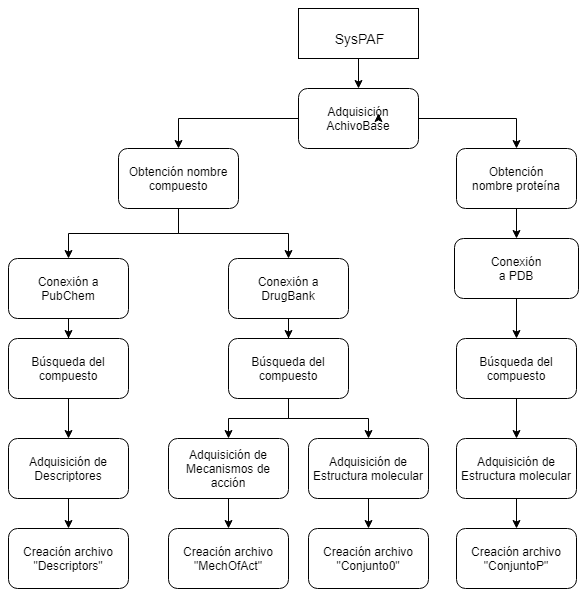
\includegraphics[scale=0.5]{Capitulo3/images/1_5Estructura.png}
    \caption{Diagrama de Estructura}
    \label{Diagramas_de_estructura}
\end{figure}

\begin{figure}[H]
    \centering
    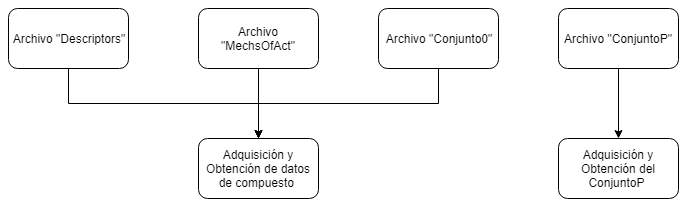
\includegraphics[scale=0.5]{Capitulo3/images/1_5EstructuraMod2.png}
    \caption{Diagrama de Estructura modulo 2}
    \label{Diagrama_Estruct_mod2}
\end{figure}
%%%%%%%%%%%%%%%%%%%%%%%%%%%%%%%5
\section{Especificación de requisitos de operación y seguridad}
\noindent El objetivo de esta tarea es definir los procedimientos de seguridad y operación
necesarios para no comprometer el correcto funcionamiento del sistema y garantizar el
cumplimiento de los niveles de servicios que exigirá el sistema en cuanto a la gestión de
operaciones (procesos por lotes, seguridad, comunicaciones, etc.).
% Please add the following required packages to your document preamble:
% \usepackage{longtable}
% Note: It may be necessary to compile the document several times to get a multi-page table to line up properly
\begin{longtable}{|l|l|l|}
\caption{Especificación de requisitos de operación y seguridad}
\label{Especificacion_de_req_op_seg}\\
\hline
\textbf{ID Requerimiento} & \textbf{Nombre}              & \textbf{Descripción}                                                                                                                                                                                                                                                    \\ \hline
\endfirsthead
%
\multicolumn{3}{c}%
{{\bfseries Tabla \thetable\ Continuación de la página anterior}} \\
\endhead
%
RFS1                      & Control de modificaciones.   & \begin{tabular}[c]{@{}l@{}}Se debe generar una\\ bitácora de la tarea a \\ realizar indicando:\\ - Actividad realizada.\\ - Indicación de módulo\\ de proceso modificado.\\ - Miembro que lo realizó.\end{tabular}                                                      \\ \hline
RFS2                      & Revisión de versiones.       & \begin{tabular}[c]{@{}l@{}}A través de la herramienta \\ Git, logrando llevar a cabo \\ un seguimiento del \\ versionado del sistema.\end{tabular}                                                                                                                      \\ \hline
RFS3                      & Acceso a Archivo             & \begin{tabular}[c]{@{}l@{}}Garantizar, que si el usuario\\ desea ver la información\\ existente en los archivos, \\ sea solo vista.\end{tabular}                                                                                                                        \\ \hline
RFS4                      & Negación de modificación     & \begin{tabular}[c]{@{}l@{}}Se debe de garantizar, que\\ los archivos donde se\\ almacene la información \\ obtenida, sea solo \\ modificada por el sistema.\end{tabular}                                                                                                \\ \hline
RFS5                      & Modificación al sistema      & \begin{tabular}[c]{@{}l@{}}El usuario, no tendrá la \\ capacidad de modificar o\\ alterar configuraciones \\ del sistema, más que \\ aspectos de visualización \\ e interfaz gráfica.\end{tabular}                                                                      \\ \hline
RFS6                      & Acceso a las bases de datos. & \begin{tabular}[c]{@{}l@{}}No habrá manera en la\\ que se modifique el \\ acceso a las bases de \\ datos para la recolección \\ de información.\\ - Cambios en la \\ dirección de la \\ base de datos.\\ - Alteración en el \\ driver para la \\ conexión.\end{tabular} \\ \hline
\end{longtable}
\section{Verificación de las Especificaciones de Diseño}
\noindent El objetivo de esta tarea es asegurar la calidad formal de los distintos modelos, conforme
a la técnica seguida para la elaboración de cada producto y a las normas y estándares
especificados en el catálogo de normas.

\begin{figure}[H]
    \centering
    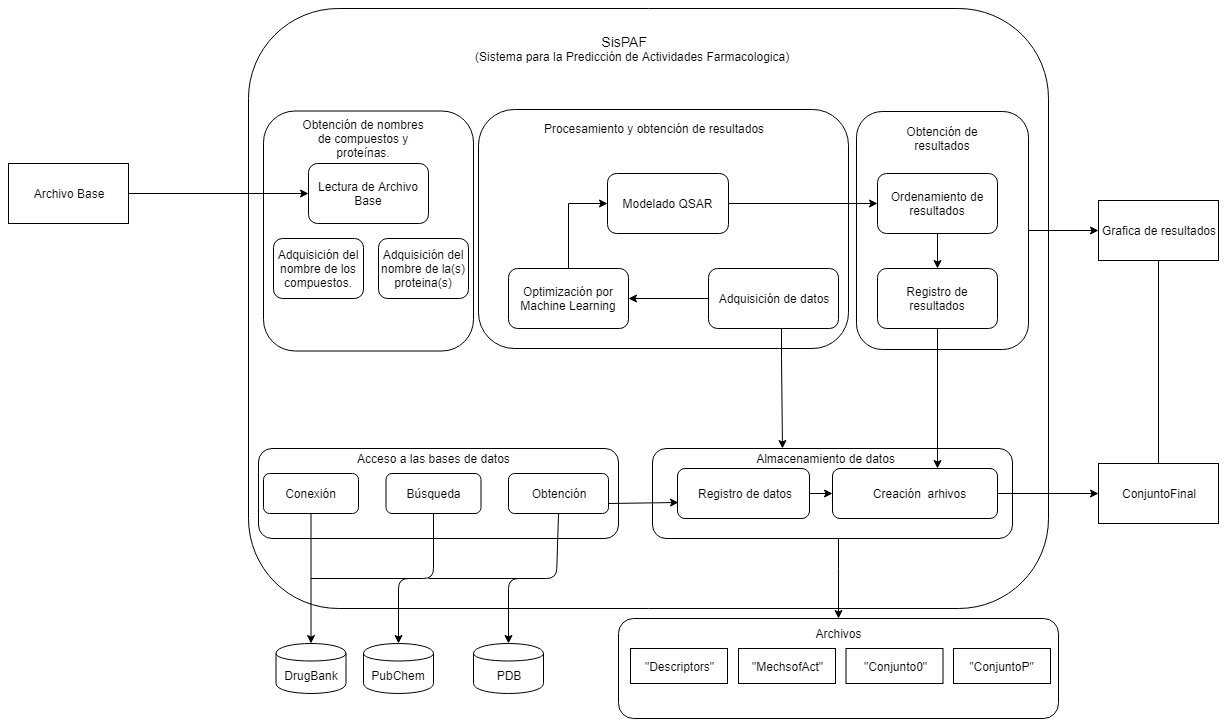
\includegraphics[scale=0.35]{Capitulo3/images/7_1.png}
    \caption{Diseño de arquitectura modular.}
    \label{Diagram_4}
\end{figure}
